\section{Bases orthonormales et frames}
\subsection{Intérêt des bases orthonormales et description des outils mathématiques disponibles}
Une approche classique et pratique pour l'analyse de signaux est l'utilisation d'une base orthonormale pour représenter un signal. 
En effet l'intérêt est multiple: si l'on connait une base orthonormale de décomposition d'un signal, il y a une unique façon d'écrire ce signal dans cette base, mais surtout, l'espace est alors naturellement muni d'un produit scalaire qui permettra d'utiliser tout l'outillage des espaces de Hilbert pour résoudre le problème.
\newline
On verra ainsi dans cette section tout d'abord des définitions et propriétés classiques des espaces de Hilbert. 
Ensuite on verra progressivement comment relacher certaines des définitions initiales afin de pouvoir conserver une formule de reconstruction.
Afin d'expliciter l'intérêt de ces définitions on verra deux exemples de frames.
Tout d'abord le frame de Fourier, dont la compréhension sera utile pour le troisième chapitre.
Ensuite, nous introduirons les ondelettes par l'analyse multi-résolution; les formules que nous obtiendrons seront utilisées pour montrer que certaines ondelettes permettent d'obtenir des formules de reconstruction avec une approximation rapide sur certaines classes de fonctions.
Ainsi, après ce chapitre il devrait être clair que la reconstruction en norme $||\cdot||_2$ est faisable, de plusieurs façons et qu'il est possible que de telles reconstructions aient une représentation parcimonieuse\footnote{En fait la représentation obtenue avec un frame n'est généralement pas exactement parcimonieuse, de nombreux coefficients peuvent avoir une petite valeur différente de 0, cependant il est possible de conserver une bonne formule de reconstruction avec moins de coefficients, soit par seuillage, soit par les techniques plus élaborées du chapitre 4}.
\subsection{Lien entre frame et base orthonormale}
Rappelons tout d'abord les définitions et propriétés d'une base orthonormale. On considère ici $H$ un espace de Hilbert donc un espace vectoriel muni d'une base hilbertienne et d'un produit scalaire.
Pour alléger les notations, on considère que $H$ est un $\mathbb{R}$-espace vectoriel, pour passer à un $\mathbb{C}$-espace vectoriel la seule modification est d'appliquer la conjugaison à de nombreux endroits.
L'ensemble des résultats présentés restent vrais dans le cas complexe.
\begin{definition}
	On dira qu'une famille $\{e_i\}_I$ d'éléments de $H$ est :
	\begin{itemize}
		\item \it{libre} si pour n'importe quelle suite finie de coefficients $(\lambda_i)_{J, J\subset I}$ telle que $\sum_J \lambda_i e_i = 0$, on a $\lambda_i = 0$ pour n'importe quel $i \in J$.
		\item \it{orthogonale} si pour n'importe quels $i$ et $j$ différents on a $\langle e_i, e_j \rangle = 0$
		\item \it{totale} si quel que soit $f \in H$ tel que pour tout $i\in I$ on a $\langle f, e_i \rangle = 0$, alors $f =0$.
		\item une \it{base hilbertienne} si la famille est orthonormale et totale.
	\end{itemize}
\end{definition}

Donc, pour tout $h \in H$, si la famille $\{e_i\}_I$ est libre et totale, il existe une unique suite $(\lambda_i)_{i \in J}$ de scalaires, telle que $ h = \sum_{i \in J} \lambda_i e_i$, on peut donc faire une identification entre $h$ et $(\lambda_i)_J$.
	On peut alors expliciter le produit scalaire sur $H$, en notant $h_1 = (\lambda_i)_J, h_2=(\mu_i)_2$
\begin{align}
	\langle \cdot, \cdot \rangle :  H \times H &\longrightarrow \mathbb{R} \\
		(h_1, h_2 ) &\longmapsto \langle h_1, h_2 \rangle = \sum_I \lambda_i \mu_i.
\end{align}
On peut remarquer que ce produit scalaire est défini de façon unique par rapport à la base hilbertienne $\{e_i\}_I$, cependant, si $U:H\rightarrow H$ est un opérateur unitaire, ce qui correspond en dimension finie à une rotation ou à un changement de base, alors on a $\langle Uh_1, Uh_2 \rangle = \langle h_1, h_2 \rangle$.
On peut donc dire que la valuation du produit scalaire ne dépend pas du choix de la base hilbertienne.
Par exemple,  en supposant connu le fait que la transformée de Fourier est un opérateur unitaire, par exemple sur $L^2(\mathbb{R})$, on a l'égalité de Plancherel avec l'égalité précédente et de celle-ci découle l'égalité de Parseval en prenant $h_1 = h_2$.
On a alors de façon générale le théorème suivant qui nous donne une condition nécessaire et suffisante pour que l'espace engendré par une famille $\{f_i\}$ soit dense dans $H$:
\begin{theoreme}
	Soit $\{f_i\}_I$ une suite d'éléments orthonormaux dans $H$ muni d'un produit scalaire.
	Alors $\overline{\text{Vect}(\{f_i\}_I)} = H$ si et seulement si 
	\begin{equation*}
		\sum_I |\langle f, f_i\rangle|^2 = ||f||^2 \quad, \forall f \in H.
	\end{equation*}
\end{theoreme}
Cependant, comme on le verra dans la suite, il y a des situations dans lesquelles chercher à avoir une base orthonormale est trop restrictif, on cherchera donc à relacher les conditions sur la définition d'une base.
\newline
Tout d'abord, si la famille est orthogonale mais n'est pas génératrice on a le résultat suivant :
\begin{theoreme}\label{th:orth1}
	Soit $\{f_i\}_I$ une famille orthonormale de $H$.
	Alors,
	\begin{equation*}
		\sum_I |\langle f, f_i \rangle|^2 \leq ||f||^2 \quad, \forall f \in H
	\end{equation*}.
\end{theoreme}
On peut exprimer ce théorème en disant que l'analyse par une famille orthogonale n'ajoute pas d'énergie au vecteur analysé.
Si la famille est génératrice,
\begin{theoreme}\label{th:norm1}
	Soit $\{f_i\}_I$ une famille génératrice normalisée.
	Alors,
	\begin{equation*}
		||f||^2 \leq \sum_I |\langle f, f_i \rangle|^2 \quad, \forall f \in H
	\end{equation*}.
\end{theoreme}
On peut exprimer ce théorème en disant que l'analyse par une famille génératrice capture au moins l'énergie du vecteur analysé, cependant elle peut ne pas en capturer toute l'énergie.
Au vu de ces résultats, on est amenés à considérer les définitions suivantes qui correspondent au fait de prendre des familles qui ne sont pas nécessairement orthogonales ou libres.
\begin{definition}
	Pour une famille d'éléments $\{f_i\}_I$ de $H$, alors on dit que c'est 
	\begin{enumerate}
		\item Une suite de \it{Bessel} si il existe une constante $M>0$ telle que
			\begin{equation*}
				\sum_I |\langle f, f_i \rangle|^2 \leq M||f||^2, \forall f \in H.
			\end{equation*}
		\item Un \it{frame} si il existe des constantes $M, m>0$ telles que
			\begin{equation}\label{eq:defFrame}
				m||f||^2 \leq \sum_I |\langle f, f_i\rangle|^2 \leq M||f||^2, \forall f \in H.
			\end{equation}
		\item Une \it{base de Riesz} (ou base \it{inconditionnelle}) si il existe des constantes $M, m>0$ telles que
			\begin{equation*}
				m\sum |c_k|^2 \leq ||\sum c_k f_k||^2 \leq M\sum |c_k|^2
			\end{equation*}
		pour n'importe quelle famille finie $\{c_k\}$.
	\end{enumerate}
\end{definition}
En utilisant les trois théorèmes précédents on a les résultats suivants: 
\begin{proposition}
	\begin{itemize}
		\item Une base orthonormale est une base de Riesz avec $m = M = 1$.
		\item Une base de Riesz est un frame dont les éléments sont linéairement indépendents.
		\item Un frame est une suite de Bessel dont les éléments sont générateurs.
	\end{itemize}
\end{proposition}

Avec ces résultats, lorsque l'on dispose d'une famille de vecteurs $F = \{f_i\}_I$ on peut définir l'opérateur d'analyse
\begin{equation*}
	\theta_F (f) = \{\langle f, f_i \rangle\}_I 
\end{equation*}
et de synthèse
\begin{equation*}
	\theta^*_F( \{c_i\}_I) = \sum_I c_i f_i.  
\end{equation*}
Ainsi la composée des deux opérateurs nous donne un opérateur de projection dans l'espace vectoriel engendré par $F$ :
\begin{equation}\label{eq:thetaF}
	\theta^*_F \circ \theta_F (f) = \sum_I \langle f, f_i\rangle f_i. 
\end{equation}
Tout d'abord on peut remarquer que, si $F$ est une famille orthonormale, alors l'application précédente correspond à une projection orthogonale dans l'espace engendré par $F$.
On va maintenant voir que si $F$ est un frame \textit{serré} (ou \textit{équilibré}) (c'est à dire avec des constantes $m, M$ égales), alors on dispose d'une formule analogue à \ref{eq:thetaF} qui nous donne une projection orthogonale.
L'intérêt de cela étant que, si $F$ est génératrice de l'espace entier $H$, alors la projection orthogonale correspond à une formule de reconstruction.
\newline
Supposons ainsi que l'on ait $m=M$, on a d'après \ref{eq:defFrame}, 
\begin{equation*}
	\sum_I |\langle f_j, f_i \rangle |^2 = M||f_j||^2.
\end{equation*}
Posons $\pi = \frac{1}{M}\theta^*_F \circ \theta$ et vérifions que c'est une projection orthogonale, soit $f\in Vect(F)$, alors
$f = \sum_J \lambda_j f_j$ avec $J\subset I$, d'où,
\begin{equation*}
	\langle f, f_k \rangle = \sum_J \lambda_j \langle f_j, f_k \rangle = \lambda_k \langle f_k, f_k \rangle + \sum_{j \in J-\{k\}} \lambda_j \langle f_j, f_k \rangle  
\end{equation*}
\begin{equation*}
	\pi(f) = \frac{1}{M}\sum_I \langle f, f_i \rangle f_i 
	= \frac{1}{M}\sum_J \lambda_j \sum_I \langle f_j, f_i \rangle f_i  
\end{equation*}
et pour conclure, on projète $\pi(f)$, sur chaque composante $f_k$ et on obtient
\begin{align*}
	\langle \pi(f), f_k \rangle &= \frac{1}{M} \sum_J \lambda_j \sum_I \langle f_j, f_i \rangle \langle f_i, f_k \rangle 
	= \frac{1}{M}  \lambda_k \sum_I |\langle f_k, f_i\rangle|^2 + \frac{1}{M} \sum_{j \in J-\{k\}}\lambda_j \sum_I  \langle f_j, f_i \rangle \langle f_i, f_k \rangle \\
	&= \frac{1}{M} \lambda_k M \langle f_k, f_k \rangle + \frac{1}{M} \sum_{j \in J-\{k\}} \lambda_j M\langle f_j, f_k \rangle \\
	&= \langle f, f_k \rangle.
\end{align*}
On a donc, si $f$ est dans l'espace engendré par F, que la projection ne change pas les coordonées de $f$. Sinon, si $f$ est dans l'orthogonal de $F$, alors chacune de ses composantes est orthogonale à tous les $f_i$, donc $f$ est dans le noyau de $\pi$.
Ainsi, $\pi$ est bien une projection orthogonale dans $F$.
\newline
On dispose donc d'une formule de reconstruction qui est valable pour tout $f$ qui est dans l'espace engendré par $F$ 
\begin{equation}
	f = \frac{1}{M} \sum_{f_i \in F} \langle f, f_i \rangle f_i .
\end{equation}
\begin{wrapfigure}{r,h}{5cm}
	\centering
	\includegraphics{Figs/frameR2}
	\caption{Le frame équilibré $\Phi = \{\varphi_1, \varphi_2, \varphi_3\}$ de $\mathbb{R}^2$}
	\label{fig:frameR2}	
\end{wrapfigure}
	
Cependant cette formule peut sembler ajouter un inconvenient avec la constante $1/M$ par rapport à la formule de reconstruction dans une base orthonormale (cas $m=M=1$ d'après la combinaison des théorèmes \ref{th:orth1} et \ref{th:norm1}). 
Nous allons voir ci-dessous en quoi avoir un coefficient de frame serré $M>1$ permet d'améliorer la stabilité de la formule de reconstruction, on appelera un tel frame un frame redondant.
Par ailleurs, une démonstration est donnée en annexe \ref{bestframe} qui montre que la solution obtenue par les coefficients de frame est la solution minimale pour la norme $\ell^2$.
\newline
En annexe \ref{recframe} une généralisation de la formule de reconstruction est donnée pour des frames non serrés, celle ci est obtenue avec un algorithme ayant une vitesse de convergence expontielle.
\newline
Avant de poursuivre vers l'étude de frames plus sophistiqués dans les parties suivantes, considérons un frame élémentaire.
	On se place dans $\mathbb{R}^2$ et on considère la famille de vecteurs $\Phi= \{\varphi_1 = (0, 1), \varphi_2 = (-\frac{\sqrt{3}}{2}, -\frac{1}{2}), \varphi_3 =(\frac{\sqrt{3}}{2}, -\frac{1}{2})\}$.
	Cette famille n'est clairement pas orthogonale, ses éléments sont libres deux à deux, mais la famille n'est pas libre (en effet, $\varphi_1 +\varphi_2 +\varphi_3 = 0$).
	Cependant, cette famille forme un frame, pour le vérifier, prenons $x=(x_1, x_2)$ un élément de $\mathbb{R}^2$, alors,
	\begin{align*}
		\sum_{i=1}^3 |\langle x, \varphi_i \rangle|^2 &= |x_2|^2 + |-\frac{\sqrt{3}}{2}x_1 -\frac{1}{2} x_2|^2 + |\frac{\sqrt{3}}{2}x_2 - \frac{1}{2}x_1|2 \\
		&= \frac{3}{2}(|x_1|^2 + |x_2|^2) = \frac{3}{2} ||x||_2^2.
	\end{align*}
	Ainsi, les vecteurs $(\varphi_1, \varphi_2, \varphi_3)$ forment un frame équilibré de constante $M=\frac{3}{2}$ de $\mathbb{R}^2$ et on a donc la formule de reconstruction :
	\begin{equation}
		x = \frac{1}{M}( \sum_{i=1}^3 \langle x, \varphi_i \rangle \varphi_i) = \frac{2}{3}( \langle x, \varphi_1 \rangle \varphi_1 +  \langle x, \varphi_1 \rangle \varphi_1   + \langle x, \varphi_1 \rangle \varphi_1) 
	\end{equation}
Ainsi, comme aperçu par Jean Morlet dès 1986 (\cite{daubch3}) travailler avec des frames permet, en pratique, de pouvoir stocker des coefficients de frame avec moins de précision, donc par exemple en mettant à 0 les coefficients proches de 0, ou bien en admettant une erreur de quantification plus importante.
\begin{remarque}\label{rq:lemmemallat}
La démonstration proposée ici poursuit l'exemple donné par Ingrid Daubechies, l'exemple présenté dans \cite{daubch3} est dans le cadre du frame \ref{fig:frameR2}, on prolonge ici ce raisonnement aux frames finis serrés arbitraires.
En cherchant à prolonger ce résultat un résultat intermédiaire était nécessaire, le lemme \ref{th:dimFrame}, une preuve originale et élémentaire est proposée ici.
Afin de vérifier que le résultat et la preuve étaient corrects, le résultat a été cherché dans la littérature publiée sur le sujet et trouvé dans le livre de Stéphane Mallat \cite{mallatframe}, théorème 5.2.
On reproduira et discutera du théorème de Stéphane Mallat qui est plus général et dont la démonstration est plus simple après la démonstration du lemme \ref{th:dimFrame}.
\end{remarque}
Voyons comment formaliser l'observation de Jean Morlet, on considère un frame $F=(f_i)_{i=1,\cdots,N}$ serré (c'est-à-dire $m=M$) redondant (c'est-à-dire $m>1$).
Ce frame engendre un espace vectoriel $Vect(F)$ de dimension $d\leq N$ car les éléments de $F$ n'ont pas à être linéairement indépendants.
Fixons un élément $f\in Vect(F)$.
Tout d'abord, exprimons $f$ dans une base orthonormale $(e_i)_{i=1,\cdots, d}$, on a ainsi la formule standard:
\begin{equation*}
	f = \sum_{i=1}^d \langle f, e_i \rangle e_i = \sum_{i=1}^d c_i e_i.
\end{equation*}
Puis perturbons les coefficients de la façon suivante: fixons un $\epsilon >0$ qui nous permettra de contrôler la taille de la perturbation introduite, et prenons $d$ variables aléatoires réelles indépendantes $(\alpha_i)_{i=1,\cdots, d}$ de moyenne nulle et de variance égale à 1.
On peut alors perturber chaque coefficient $c_i$ en y ajoutant $\epsilon \alpha_i$, on peut alors calculer l'erreur de reconstruction moyenne
\begin{align*}
	\mathbb{E}\left(|| f- \sum_{i=1}^d (c_i + \epsilon \alpha_i)e_i||_2^2\right) &= \mathbb{E}\left(\sum_{i=1}^d \epsilon^2 \alpha_i^2\right)\\
		&= \epsilon^2 \sum_{i=1}^d \mathbb{E} (\alpha_i^2) = \epsilon^2 d \label{eq:errorth}.
\end{align*} 
Ensuite, appliquons la même altération aux coefficients de $f$ dans le frame $F$ afin de calculer l'erreur de reconstruction moyenne.
Considérons la formule de reconstruction
\begin{equation*}
	f = \frac{1}{M}\sum_{i=1}^N \langle f, f_i \rangle f_i
\end{equation*}
et prenons $N$ variables aléatoires réelles indépendantes $(\alpha_i)_{i=1, \cdots, N}$  de moyenne nulle et de variance égale à 1.
\begin{align}
	\mathbb{E}\left(|| f- \frac{1}{M}\sum_{i=1}^N (\langle f, f_i\rangle + \epsilon \alpha_i)f_i||_2^2\right) &= \mathbb{E}\left(||\frac{1}{M} \sum_{i=1}^N \epsilon \alpha_i||_2^2\right)\nonumber\\
	&= \frac{\epsilon^2}{M^2} \mathbb{E}(\sum_{i=1}^N \alpha_i^2) = \frac{\epsilon^2}{M^2} \sum_{i=1}^N \mathbb{E}(\alpha_i^2) \nonumber\\
	&= \frac{\epsilon^2 N}{M^2} \label{errframe}%%TODO Enlever dernière ineq 	
\end{align}
Si on souhaite comparer les majorations obtenues dans le cas orthonormal et dans le cas d'un frame serré, il nous faut donc une relation entre : le nombre d'éléments dans un frame serré ($N$), la constante de frame ($M$) et la dimension de l'espace engendré par le frame ($d$).
\begin{lemme}\label{th:dimFrame}
	Soit $\Phi =(\varphi_i)_{i=1, \cdots, N}$ un frame avec des constantes de frame $m=M$ qui engendre $Vect(\Phi)$ un espace vectoriel de dimension $d$.
	Alors
	\begin{equation}
		\frac{N}{M} \leq d.
	\end{equation}
\end{lemme}
Avec ce lemme, on peut donc comparer l'erreur de reconstruction moyenne après perturbation dans le cas d'un frame \ref{errframe} et dans le cas d'une base orthonormale:
\begin{equation}
	\frac{N}{M^2} \leq \frac{\epsilon^2d}{M} < \epsilon^2 d.
\end{equation}
Ainsi, en revenant au cas du frame de $\mathbb{R}^2$ \ref{fig:frameR2}, on a que si on perturbe les coefficients l'erreur de reconstruction est améliorée d'un facteur $\frac{2}{3}$ par rapport à celle que l'on obtiendrait en utilisant une base orthonormale de $\mathbb{R}^2$.
Maintenant passons à la preuve originale du lemme:
\begin{proof}
	Afin de prouver ce résultat rappelons que l'on a l'opérateur d'analyse
	\begin{align}
		A :	\mathbb{R}^d &\longrightarrow \ell^2(N)\\
			f &\longmapsto (\langle f, \varphi_i \rangle)_{i=1,\cdots, N}
	\end{align}
	et le frame étant équilibré, la boule $B_d(0,1)$ dans $\mathbb{R}^d$ de rayon 1 est envoyée sur la boule $B_N(0,M)$ de $\ell^2(N)$.
	Maintenant, on considère l'opérateur de synthèse,
	\begin{align}
		S :	\ell^2(N) &\longrightarrow^S \mathbb{R}^d\\
			x=(x_i)_{i=1, \cdots, N} &\longmapsto \sum_{i=1}^N x_i \varphi_i
	\end{align}
	et on considère, sans perte de généralité que chaque $\varphi_i$ est normalisé. Ainsi chaque à chaque $\varphi_i$, on peut associer une suite $(\lambda_j^i)_{j=0, \cdots, d}=(\langle \varphi_i, e_j\rangle)_{j=0,\cdots, d}$ de norme 1 dans $\mathbb{R}^d$ muni de la norme euclidienne telle que $\varphi_i = \sum_{j=1}^d \lambda_j^i e_j$ où $e_j$ est une base orthonormale de $\mathbb{R}^d$. 
	L'objectif est maintenant de réécrire $S(x)$ dans la base orthonormale, on a ainsi
	\begin{equation}
		\sum_{i=1}^N x_i \varphi_i = \sum_{i=1}^N x_i \sum_{j=1}^d \lambda_j^i e_j = \sum_{j=1}^d \sum_{i=1}^N x_i \lambda_j^ie_j =\sum_{j=1}^d c_j e_j,
	\end{equation}
	où $c_j = \sum_{i=1}^Nx_i\lambda_j^i$. On va maintenant majorer les $c_j$ de façon uniforme, chaque $\lambda_j^i$ correspond à la projection de $\varphi_i$ sur $e_j$, chaque $\varphi_i$ est dans la boule unité ainsi $c_j$ correspond à la projection de tous les $\varphi_i$ sur $e_j$, ainsi on a avec l'inégalité de Cauchy-Schwarz la majoration
	\begin{equation}
		c_j \leq ||x||_2 \sqrt{M}.
	\end{equation}
	On a maintenant la majoration,
	\begin{equation}
		||S (x)||^2_2 = ||\sum_{j=1}^d c_j e_j||_2^2= \sum_{j=1}^d c_j^2 \leq d M||x||_2^2. 
	\end{equation}
	On va maintenant chercher une minoration de $||S(x)||_2^2$,
	\begin{equation}
		||S(x)||_2^2 = ||\sum_{i=1}^N x_i \sum_{j=1}^d \lambda_j^i e_j||_2^2 \geq N||x||_2^2 \min_{i=1, \cdots, N} ||\sum_{j=1}^d \lambda_j^i e_j||_2^2 = N||x||_2^2 \min_{i=1, \cdots, N}\sum_{j=1}^d (\lambda_j^i)^2.
	\end{equation}
	Or,
	\begin{equation}
		\sum_{i=1}^d (\lambda_j^i)^2 = \sum_{i=1}^d |\langle \varphi_j, e_i \rangle|^2 =||\varphi_j||_2^2=1.  
	\end{equation}
	On peut donc combiner les inégalités obtenues et on a
	\begin{equation}
		N ||x||_2^2 \leq ||S(x)||_2^2 \leq d M||x||_2^2
	\end{equation}
	et ainsi
	\begin{equation}
		\frac{N}{M} \leq d.
	\end{equation}
\end{proof}
Comme discuté dans la remarque \ref{rq:lemmemallat}, un résultat plus général est présenté dans le livre de Stéphane Mallat \cite{mallatframe}, le voici:
\begin{theoreme}[Mallat]
	Soit $\Phi =(\varphi_i)_{i=1, \cdots, N}$ un frame avec des constantes de frame $m,M$ qui engendre $Vect(\Phi)$ un espace vectoriel de dimension $d$.
	Alors
	\begin{equation}\label{eq:eqmallat}
		m \leq \frac{N}{d} \leq M.
	\end{equation}
	Si le frame est serré, $m=M=\frac{N}{d}$.
\end{theoreme}
Premièrement, remarquons que la dernière égalité est une conséquence de l'inégalité avec $m=M$.
\newline 
Ensuite, remarquons que l'on peut réécrire \ref{eq:eqmallat} de façon équivalente:
	\begin{equation}
		d \leq \frac{N}{m} \quad \text{et} \quad \frac{N}{M} \leq d.
	\end{equation}
	La deuxième inégalité étant celle du lemme \ref{th:dimFrame}, pour passer de ce lemme au théorème précédent, il faut donc montrer que cette inégalité dans le cas d'un frame qui n'est pas équilibré.
	En étudiant la preuve du lemme qui est donnée ici, on voit que le fait que le frame soit équilibré intervient dans la première partie, dans laquelle on cherche une majoration.
	Comme on cherche une majoration, en étudiant la preuve on peut voir qu'elle fonctionne aussi si $m\leq M$.
	Donc pour arriver au résultat de Stéphane Mallat, il reste à montrer l'inégalité
	\begin{equation}
		d \leq \frac{N}{m}.
	\end{equation}
	On peut se convaincre, et montrer, qu'une preuve très similaire à celle du lemme est possible qui permet de prouver cette dernière inégalité et le théorème de Stéphane Mallat.
	En effet, il y a certaines symétries que l'on peut utiliser pour obtenir les inégalités dans l'autre sens. 
	Il semble donc qu'un argument plus général puisse exister pour faciliter cette preuve.
	On présente donc la preuve de Stéphane Mallat qui utilise naturellement la trace d'un opérateur et les valeurs propres.
	\begin{proof}
		Remarquons tout d'abord que la définition de l'opérateur de synthèse $S$ par rapport à $A$ que l'on fait ici correspond exactement à prendre l'opérateur adjoint de $A$, que l'on note $A^*$.
		Celui-ci vérifie pour tout $f\in Vect(F)$ et pour tout $x\in Im(A) \subset \ell^2(N)$,
		\begin{equation}
			\langle Af, x \rangle = \langle f, A^*x \rangle.
		\end{equation}
		On peut alors remarquer
		\begin{equation}
			||Af||^2 = \sum_{i=1, \cdots,N} \langle f, f_i \rangle^2 = \langle A^*Af, f\rangle.
		\end{equation}
		On peut donc réécrire la condition de frame \ref{eq:defFrame} sous la forme:
		\begin{equation}
			m||f||^2 \leq \langle A^*Af, f\rangle \leq M||f||^2.
		\end{equation}
		On voit alors que les bornes de frame $m$ et $M$ correspondent à la plus petite et à la plus grande valeur propre de $A^*A$ en dimension finie, aussi appelées valeurs singulières de $A$.
		\newline
		On peut maintenant prouver le théorème en quelques lignes : les valeurs propres de $A$ sont donc entre $m$ et $M$, ainsi
		\begin{equation}\label{eq:traceeq}
			dm \leq Tr(A^*A) \leq dM
		\end{equation}
		car $A^*A$ agit sur un espace isométrique à $\ell^2(d)$.
		En utilisant le fait que $Tr(A^*A) = Tr(AA^*)$, on a:
		\begin{equation}
			Tr(AA^*) = \sum_{i=1,\cdots, N} |\langle f_i, f_i \rangle|^2 = N
		\end{equation}
		et on a alors prouvé le théorème en insérant le précédent résultat dans \ref{eq:traceeq}.  	
	\end{proof}	
	En comparant cette preuve et celle du lemme, on voit que la trace permet de concentrer le raisonnement du lemme en quelques lignes.
	On voit alors l'efficacité de la trace et l'importance des valeurs propres pour prouver ce type de résultat.
	Ainsi, certains des raisonnements dans la suite de ce mémoire utiliseront ce point de vue spectral.
	\newline
	Avant de poursuivre vers des exemples de frames, remarquons que dans cette partie un point de vue plus général aurait pu être possible.
	En effet, on aurait pu considérer travailler dans des espaces de Banach plutôt que de Hilbert, on aurait pu introduire d'autres notions de bases telles que les bases de Hamel, Schauder, Auerbach ou Markushevich plûtot que de Riesz ou Hilbert.
	On pourra consulter \cite{jaffardondelettes} notamment pour le lien qui est fait entre les définitions de ces bases et leurs liens avec les ondelettes.
	Le choix de travailler dans un espace de Hilbert a été fait car c'est un cadre suffisant pour le reste du mémoire avec des propriétés très similaire en dimension finie et infinie.
	Il est important de remarquer que ces choix ont de l'importance seulement en dimension infinie, les notions étant équivalentes en dimension finie.

\begin{wrapfigure}{r,h}{6cm}
	\centering
	\includegraphics{Figs/haar}
	\label{fig:haar}	
\end{wrapfigure}
	
	Cependant des généralisations auraient pû être possible en utilisant des notions plus restrictives, cela est notamment motivé par le fait que certaines ondelettes, par exemple, celle de Haar peuvent fournir une base raisonnable (de Schauder) de $L^p([0,1])$, pour tout $1 \leq p < \infty$, contrairement à la base de Fourier qui n'est pas une base raisonnable pour $p=1$.
	Ici on dit que la base de Fourier n'est pas raisonnable car il existe des fonctions dans $L^1([0,1])$ dont la série de Fourier ne converge pas en norme $L^1$.
	\newline
	Il semble qu'une façon par laquelle on aurait pu généraliser l'étude d'opérateurs ayant des propriétés similaires aux frames dans des espaces de Banach aurait été de donner une place centrale à la trace, en considérant la classe des opérateurs à trace, aussi appelés opérateurs nucléaires.
	A cette théorie on peut associer le nom de Grothendieck avec l'article \cite{groth}. 
	Pour une introduction aux opérateurs à trace par les frames on peut consulter \cite{traceclass}, par leur similarité à l'analyse complexe on peut consulter \cite{acQuef}, pour un point de vue historique sur leur développement on peut consulter \cite{surlestraces}. 
\subsection{Frames d'ondelettes et analyse multi-résolution}\label{sec:frameondelette}
Historiquement, au début du XXème siècle, le problème de la non-convergence de la série de Fourier de certaines fonctions continues amena David Hilbert à se demander si ce phénomène était inhérent aux bases orthogonales de $L^2([0,1])$.
C'est ainsi que sous sa direction Alfréd Haar introduit dans sa thèse \cite{haar} en 1909 la base orthogonale de $L^2([0,1])$ donnée par \ref{fig:haar}.
Jusqu'aux années 1980, aucune autre ondelette n'a été trouvée, c'est sous l'impulsion des travaux de Jean Morlet et Alexandre Grossman que le domaine des ondelettes a commencé à être exploré.
Ensuite Yves Meyer a reconnu dans leurs travaux des formules analogues à des résultats d'analyse harmonique, cependant à ce moment là, tous les frames d'ondelettes qui étaient construits étaient redondants.
Yves Meyer (voir \cite{daubpers} pour plus de détails sur l'ensemble de ces développements) a donc souhaité prouver que c'était nécessaire que les frames d'ondelettes soient redondants, et donc pas orthonormaux.
En essayant de prouver cela par l'absurde, en supposant l'existence d'un frame d'ondelette orthonormal, au lieu d'obtenir une contradiction il obtint une construction d'une famille d'ondelettes orthonormales \cite{meyer}.
A partir de là de nombreuses constructions d'ondelettes fûrent faites avec différentes propriétés de régularité, de support, de décroissance,... 
Mentionnons tout de même la construction d'ondelettes avec des moments nuls à support compact par Ingrid Daubechies \cite{daubbook} ainsi que l'algorithme de transformée en ondelette discret et le concept d'analyse multi-résolution de Stéphane Mallat \cite{mallatbook} qui ont permis aux ondelettes de devenir un outil maintenant très répandu dans les mathématiques appliquées et que l'on utilisera dans la suite du mémoire.
Les concepts d'analyse-temps fréquence et de localisation développés dans la théorie des ondelettes sont aujourd'hui développés en mathématiques pures dans le cadre de l'analyse micro-locale. On pourra à nouveau consulter \cite{jaffardondelettes} pour un exposé général sur le développement et le rôle des ondelettes dans les mathématiques actuelles.
\newline
Etudions donc ces ondelettes:
\begin{definition}
	On dit que $\psi:\mathbb{R} \to \mathbb{R}$ est une ondelette génératrice si 
	\begin{equation}
		\{\psi_{j,k} := 2^{j/2}\psi(2^j\cdot - k)\}_{j,k \in \mathbb{Z}}
	\end{equation}
	est une famille génératrice de $L^2(\mathbb{R})$.
	On appelera\footnote{On considérera par la suite des frames d'ondelettes ou bien des bases de Riesz d'ondelettes} une base engendrée par une telle fonction $\psi$ une base d'ondelettes.
\end{definition}
\begin{figure}
	\floatbox[{\capbeside\thisfloatsetup{capbesideposition={left,top},capbesidewidth=4cm}}]{figure}[\FBwidth]
	{\caption{L'ondelette $\psi(t) = 2sinc(2t) - sinc(t)$ dite de Shannon avec différentes dilatations dyadiques $\psi_j$. Lorsque $j$ augmente, la fonction est parcourue plus rapidement d'un facteur $2^j$.}}
	{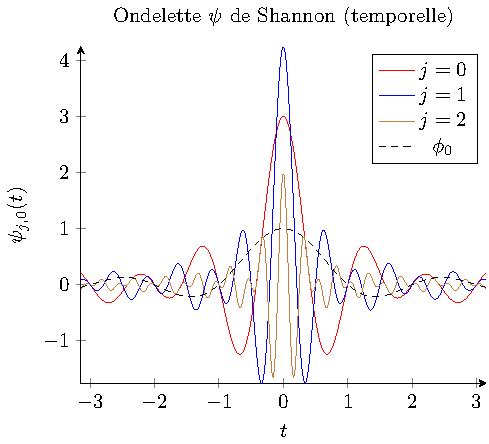
\includegraphics{Figs/shannon}}
	\label{fig:shannon}
	\floatbox[{\capbeside\thisfloatsetup{capbesideposition={right,bottom},capbesidewidth=4cm}}]{figure}[\FBwidth]
		{\caption{Des versions translatées $\psi_{j,k}$ des ondelettes $\psi_j$ du graphe précédent. Lorsque $j$ augmente, la fonction est parcourue plus rapidement d'un facteur $2^j$.}}
	{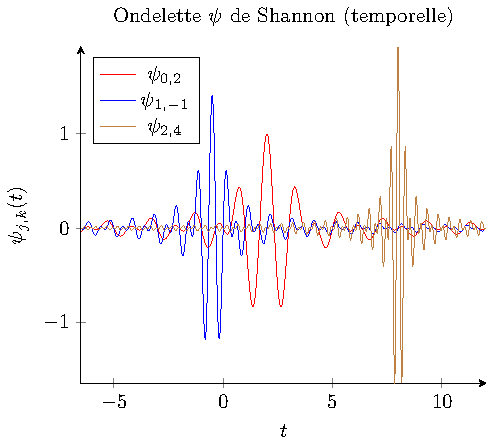
\includegraphics{Figs/shannonspat}}
\end{figure}
\begin{figure}
	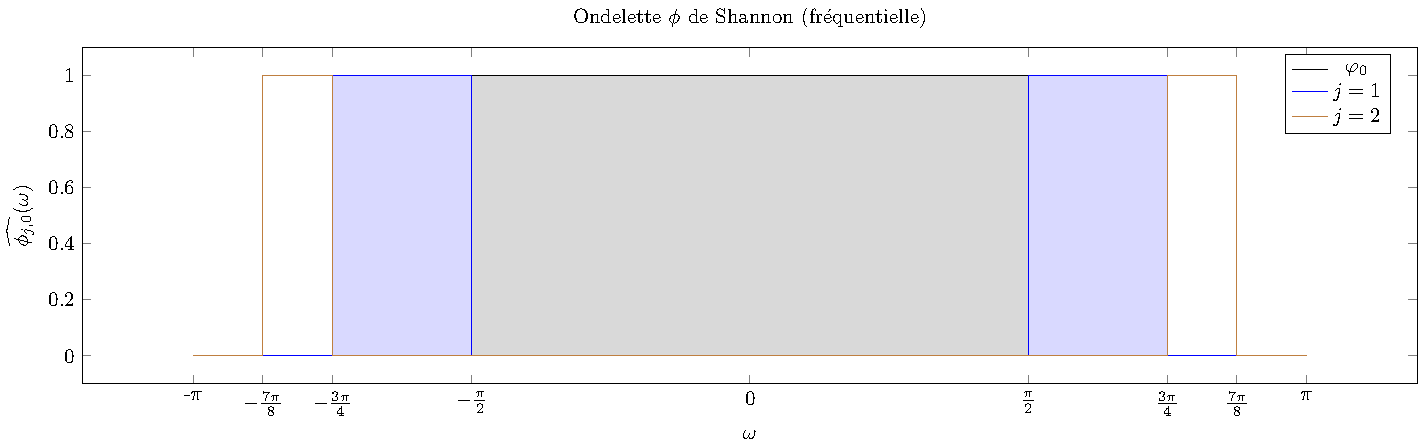
\includegraphics[width=17cm]{Figs/shannonfreq}
	\caption{La transformée de Fourier $\hat{\psi}$ de l'ondelette de Shannon $\Psi$. L'ondelette d'échelle $\phi_0$ est un filtre passe-bande $[-\frac{\pi}{2}, \frac{\pi}{2}]$, les ondelettes $ \psi_j$ sont des filtres passe bande qui recouvrent le reste de l'intervalle avec des supports disjoints de taille $2^{-j}$. On peut ainsi vérifier toutes les propriétés de l'analyse multi-résolution pour l'ondelette de Shannon sur les fonctions à bande limitée (c'est à dire, dont le support de la transformée de Fourier est borné).
	}
\end{figure}
\begin{remarque}
	Dans la définition des ondelettes $\psi_{j,k}$ engendrées par $\psi$, le coefficient $j$ correspond au facteur d'échelle\footnote{Du point de vue des notations, on considère que $j$ tend vers l'infini, signifie que $\psi_j$ analyse les hautes fréquences, ce choix de notation n'est pas uniforme dans la littérature, par exemple Stéphane Mallat et Ingrid Daubechies, utilisent $-j$ par rapport à nos notations. Par contre les notations utilisées correspondent à celles de Stéphane Jaffard et Yves Meyer. Mais cependant tous les résultats sont bien entendu équivalents.},
	en raison du facteur $2^j$ devant la variable, au fur et à mesure que $j$ augmente, l'ondelette est parcourue de plus en plus vite. Ainsi, augmenter $j$ revient à augmenter la fréquence de $\psi$, c'est à dire d'éloigner le support de $\hat{\psi}$ de l'origine. 
	Le coefficient $k$ correspond à une translation de l'ondelette $\psi_j$, en ce sens, l'analyse par ondelette, permet une analyse à la fois en temps (par rapport à $k$) et en fréquence (par rapport à $j$).
	\newline 
	En effet, de façon plus précise et formelle, on a par l'action de la transformée de Fourier sur les dilatations: 
	\begin{equation}
		\widehat{\psi_{j,0}}(\omega) = 2^{-\frac{j}{2}}\hat{\psi}(\frac{\omega}{2^j})
	\end{equation}
	et par l'action de la transformée de Fourier sur les translations:
	\begin{equation}
		\widehat{\psi_{j,k}}(\omega) = 2^{-\frac{j}{2}}\hat{\psi}(\frac{\omega}{2^j})e^{-2i\pi 2^{-j}k\omega}.
	\end{equation}
	On peut voir que l'analogie temps-fréquence dans le cadre des ondelettes implique en un certain sens le point de vue temps-fréquence de l'analyse Fourier.
	En effet, si on prend $\psi$ l'ondelette de Shannon (voir \ref{fig:shannon}), alors sa transformée de Fourier $\hat{\psi}$ est la fonction indicatrice sur $[-2\pi, \pi]\cup[\pi, 2\pi]$.
	Donc, à échelle $j$ fixée, on a que $\widehat{\psi_{j,k}}$ est supporté sur $B_j := [-2\pi2^{j+1}, -\pi2^j]\cup[\pi2^j, \pi2^{j+1}]$ et vaut:
	\begin{equation}
		\widehat{\psi_{j,k}}(\omega) = 2^{-\frac{j}{2}}e^{-2i\pi 2^{-j}k\omega}.
	\end{equation}
	Regardons maintenant la projection de $f\in L^2(\mathbb{R})$ sur les translatés de $\psi_j$, on a:
	\begin{equation}
		\langle f, \psi_{j,k} \rangle = \langle \hat{f}, \widehat{\psi_{j,k}} \rangle = \int_{B_j} \hat{f}(\omega) 2^{-\frac{j}{2}} e^{2i\pi2^{-j}k\omega} d\omega
	\end{equation}	
	donc en sommant par rapport à $k$ on a que la projection à $j$ fixé correspond à un développement en série de Fourier de $f$ avec les fréquences dans $B_j$.
	Donc l'intuition que lorsque $j$ augmente, la fréquence augmente, coincide exactement avec la notion de fréquence de la théorie de Fourier lorsque on considère l'ondelette de Shannon.

\end{remarque}
Donc étant donnée une famille d'ondelettes $\{\psi_{j,k}\}_{j,k \in \mathbb{Z}}$, comme on l'a vu on peut associer à une fonction $f\in L^2(\mathbb{R})$, ses coefficients d'ondelettes
\begin{equation}
	Wf = (\langle f, \psi_{j,k} \rangle )_{j,k \in \mathbb{Z}}
\end{equation}
et on se demande alors si à partir de ces coefficients on peut reconstruire $f$.
\begin{figure}[h]
	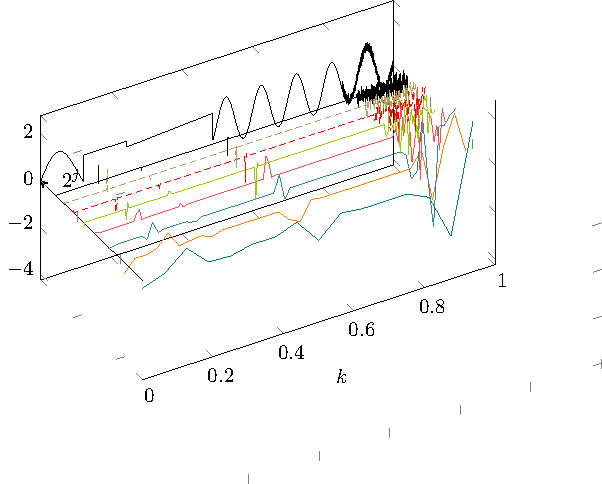
\includegraphics{Figs/wavelet}
	\caption{Les coefficients d'ondelette (pour l'ondelette de Daubechies D4) d'un signal présentant des zones de différentes régularité. Les coefficients les plus proches du signaux correspondent aux échelles les plus fines. On remarque que ces coefficients sont très petits dans les zones sans discontinuités. On peut voir que les hautes valeurs de ces coefficients (proches des discontinuités) se propagent vers les plus grandes échelles en s'étalant.}
\end{figure}
Cela revient ainsi à déterminer si la famille d'ondelettes est un frame d'ondelette. 
Ici on ne cherchera pas a énumérer et a vérifier des frames d'ondelettes, un très grand nombre de frames d'ondelettes existent\footnote{Pour une introduction au sujet des ondelettes par les frames on peut recommander le livre d'Ingrid Daubechies \cite{daubbook}, pour un théorème donnant une construction simple d'ondelettes en dimension $d\geq 1$ avec un échantillonage arbitraire (au lieu de l'échantillonage dyadique) on peut consulter \cite{IrregWav} et pour une liste d'ondelettes \url{https://en.wikipedia.org/wiki/Wavelet#List_of_wavelets}}, on admet ainsi l'existence des frames d'ondelettes. 
\newline
Supposons ainsi que l'on dispose d'un frame d'ondelettes et que ce frame est équilibré (c'est à dire que les bornes de frame $m$ et $M$ sont égales), alors on dispose d'une formule de reconstruction (d'après Daubechies 3.2.2)
\begin{equation}
	f = \frac{1}{M} \sum_{j,k} \langle f, \psi_{j,k}\rangle \psi_{j,k}.
\end{equation}
Cependant bien que la formule précédente permette une reconstruction elle suppose de parcourir des indices sur $\mathbb{Z}$ ce qui pourrait créer des complications concernant la convergence (d'un point de vue théorique ou pratique).
On va ici très rapidement introduire la notion d'analyse multi-échelle qui permet de simplifier la formule de reconstruction.
Construisons ici une analyse multi-échelle (ici de $L^2(\mathbb{R})$), considérons tout d'abord une suite d'espaces emboités satisfaisant 
\begin{equation*}
	\{0\}=	\lim_{j\to -\infty} \bigcap_{j}^{+\infty} V_i \subset \cdots \subset V_{-1} \subset V_0 \subset \cdots V_i \subset V_{i+1} \subset \cdots \subset \lim_{j\to \infty} \bigcup_{-\infty}^{j} V_i = L^2(\mathbb{R}).  
\end{equation*}
L'intérêt d'avoir une telle suite d'espaces emmboités est que étant donnée une fonction $f\in L^2(\mathbb{R})$, on peut considérer sa projection orthogonale dans un $V_i$, on a alors une approximation $f_i$ de $f$ dans $V_i$, si on souhaite améliorer l'approximation de $f$ il suffit alors de remonter dans ces espaces emboités pour avoir une reconstruction avec une précision arbitraire.
Introduisons maintenant la propriété qui va permettre de voir cette suite d'espaces comme une analyse multi-échelle
\begin{equation}
	f(\cdot) \in V_j \iff f(\frac{\cdot}{2^j}) \in V_0,
\end{equation}
c'est à dire que les fonctions d'un espace $V_j$ sont des versions dilatées d'un facteur $2^{-j}$ des fonctions de l'espace $W_0$.
Ajoutons maintenant la condition que $V_0$ contient toutes les translations entières de ses éléments, c'est à dire
\begin{equation}
	f \in V_0 \iff f(\cdot - n) \in V_0 \forall n \in \mathbb{Z}.
\end{equation}
Ainsi, une fonction qui appartient à $V_j$ s'écrit comme une combinaison linéaire de versions translatées et dilatées de fonctions appartenant à $V_0$.
De plus, quelque soit $j$ on peut prendre $W_j$ le complémentaire orthogonal de $V_j$ dans $V_{j+1}$, 
\begin{equation}
	f = \pi_{V_0}(f) +\sum_{i>0} \pi_{W_j}(f) 
\end{equation}
donc afin d'avoir une formule de reconstruction, il suffit de connaitre un frame de $V_0$ et de même pour chaque $W_j$. 
On peut maintenant revenir aux ondelettes, on considère que l'on connait $\varphi \in L^2(\mathbb{R})$ tel que $(\varphi_{k})_{k\in \mathbb{Z}}$, en notant $\varphi_k$ les translatés par $k$ de $\varphi$, soit une base de $V_0$ et $(\psi_{j,k})_{j\in \mathbb{N}^*, k \in \mathbb{Z}}$ un frame de l'orthogonal de $V_0$ dans $L^2(\mathbb{R})$, on pose alors $W_j = W_{j-1} \bigoplus Vect(\{\psi_{j,k}\}_{k\in \mathbb{Z}})$ et on obtient ainsi que l'analyse multi-échelle ainsi construite fournit une formule de reconstruction\footnote{Dans la formule de reconstruction les deux sommes sur $\mathbb{Z}$ ne sont pas problématiques car les fonctions considérées sont dans $L^2(\mathbb{R})$ donc avec une décroissance suffisament rapide, donc seulement un nombre fini de $\langle f, \varphi_{0,k} \rangle$ sont différents de 0 si $\varphi_0$ a une décroissance suffisament rapide (et de même pour chaque $\psi_j$).}
\begin{equation}
	f = \sum_{k\in \mathbb{Z}} \langle f, \varphi_{k} \rangle \varphi_{k} + \sum_{j = 1}^{+\infty} \sum_{k\in \mathbb{Z}} \langle f, \psi_{j,k} \rangle \psi_{j,k}.
\end{equation}
On appelle l'application $\varphi_0$ ondelette d'échelle.

\section{Décroissance des coefficients et régularité}
\subsection{Approximation linéaire et régularité}
On s'intéresse dans cette partie au lien entre une fonction $f\in L^2(]0, 1[)$ et son approximation dans une base. On verra un résultat reliant la décroissance des coefficients de la fonction dans une base fixée et la vitesse de convergence de la reconstruction. 
On verra ensuite à l'aide de ce résultat, que pour la base de Fourier (et resp. certaines bases d'ondelettes), on obtient des formules de reconstruction pour les fonctions dérivables (et resp. pour les fonctions Lipschitziennes) avec une erreur de reconstruction qui décroit rapidement.
\newline 
On considère ainsi un espace d'approximation de fonctions $U_N \subset L^2([0, 1])$.
Par construction, la meilleure approximation linéaire de $f$ dans $U_N$, est la projection orthogonale $f_N$ de $f$ dans $U_N$, qui peut être obtenue à l'aide de la base biorthogonale de synthèse associée $(\tilde{\phi}_k)_{k=1, \cdots, N}$ et la formule de reconstruction :
\begin{equation}
	f_N = \sum_{k=0}^{N-1}\langle f, \phi_k \rangle \tilde{\phi}_k.
\end{equation}
Afin de mesurer l'erreur d'approximation par rapport à $f$, on considère une base $\mathcal{B} = \{g_k\}_{k\in \mathbb{N}}$ de l'espace $L^2([0, 1])$ entier à laquelle on ajoute la condition de contenir une famille $(g_k)_{k\in I}$, avec $\#I = N$ qui forme une base de l'espace d'approximation $U_N$.
On peut ainsi écrire, en réordonnant la famille $(g_k)$,  $f_N \in U_N$ dans cette base :
\begin{equation}
	f_N = \sum_{k=0}^{N-1} \langle f, g_k \rangle g_k 
\end{equation}
et les $\{g_k\}_{\mathbb{N}}$ formant une base de $L^2([0, 1])$, on peut écrire $f$ dans cette base:
\begin{equation}
	f = \sum_{k=0}^{+\infty} \langle f, g_k \rangle g_k.
\end{equation}
On obtient donc que la partie orthogonale à la famille $\{\phi_k\}_{k=0, \cdots, N-1}$, est celle analysée par $\{g_k\}_{k\geq N}$.
C'est à dire, 
\begin{equation}
	f - f_N = \sum_{k=N}^{+\infty} \langle f, g_k \rangle g_k 
\end{equation}
et la mesure de l'erreur d'approximation avec $N$ coefficients est donc 
\begin{equation}
	\varepsilon_l(N, f) = ||f-f_N||^2 = \sum_{k=N}^{+\infty} |\langle f, g_k\rangle|^2.
\end{equation}
Comme on a supposé que $f\in L^2([0, 1])$ et que la famille $(g_k)$ est génératrice, on a que l'erreur d'approximation tend vers $0$ lorsque $N$ augmente.
On va maintenant s'intéresser au théorème suivant de Stéphane Mallat qui relie la décroissance des coefficients de $f$ dans la base de $L^2([0, 1])$ à la vitesse de décroissance de l'erreur d'approximation de la fonction.
\begin{theoreme}
	Soit $r > 1/2$, il existe des constantes $A, B > 0$ telles que si 
	\begin{equation}
		\sum_{k=0}^{+\infty} |k|^{2r}|\langle f, g_k \rangle |^2 < \infty,
	\end{equation}
	alors on a 
	\begin{equation}\label{eq:regframe}
		A \sum_{k=0}^{+\infty} k^{2r}|\langle f, g_k \rangle |^2 \leq 
		\sum_{N=0}^{+\infty} N^{2r-1} \varepsilon_l(N, f) \leq
		B \sum_{k=0}^{+\infty} k^{2r} |\langle f, g_k\rangle |^2
	\end{equation}
	et ainsi on a $\varepsilon_l(N, f) = o(N^{-2r})$.
\end{theoreme}
\begin{proof}
	On développe le terme au centre de l'égalité dela façon suivante 
	\begin{equation*}
		\sum_{N=0}^{\infty} N^{2r-1} \varepsilon_l(N, f) =
		\sum_{N=0}^{\infty} \sum_{k=N}^{\infty} N^{2r-1} |\langle f, g_k \rangle |^2 =
		\sum_{k=0}^{+\infty} |\langle f, g_k \rangle |^2 \sum_{N=0}^{k} N^{2r-1}.
	\end{equation*}
	Puis on majore des deux côtés avec 
	\begin{equation}
		\int_{0}^M x^{2r-1} dx \leq \sum_{N=0}^m N^{2r-1} \leq \int_{1}^{m+1} x^{2r-1}dx.
	\end{equation}
	En calculant les deux intégrales on déduit 
	\begin{equation}
		A m^{2r} \leq \sum_{N=0}^{m} N^{2r-1} \leq B m^{2r}
	\end{equation}
	où $A$ et $B$ dépendent seulement de $r$, ce qui nous donne \ref{eq:regframe}.
	Montrons maintenant $\varepsilon_l(N, f) = o(N^{-2r})$, remarquons tout d'abord que $\varepsilon_l(N, f)$ est décroissant par rapport à la première variable, on déduit de cela
	\begin{equation*}
		\varepsilon_l(N, f)\sum_{m=N/2}^{N-1} m^{2r-1} \leq \sum_{m=N/2}^{+\infty} m^{2r-1} \varepsilon_l(m, f)
	\end{equation*}
	on a donc avec le calcul précédent que le terme de droite converge quel que soit le choix de $N$, et ainsi
	\begin{equation*}
		\lim_{N \to +\infty} \sum_{m=N/2}^{+\infty} m^{2r-1}\varepsilon_l(m, f) = 0
	\end{equation*}
	donc tous les termes de l'inégalité précédente tendent vers 0. 
	De plus, $\sum_{m = N/2}^{N-1} m^{2r-1} \geq CN^{2r}$ et donc
	\begin{equation*}
		\lim_{N\to \infty} \varepsilon_l(N, f)N^{2r} = 0.
	\end{equation*}
\end{proof}
On a ainsi démontré que si $f$ appartient à l'espace
\begin{equation}
	W_{\mathcal{B}, r} =\{f : \sum_{m=0}^{+\infty} m^{2r} |\langle f, g_m \rangle |^2 < \infty\}
\end{equation}
alors l'approximation linéaire dans la base $\mathcal{B}$ décroit au moins comme $N^{-2r}$.
On montrera dans la prochaine sections que si $\mathcal{B}$ est une base de Fourier alors $W_{\mathcal{B}, r}$ contient les fonctions $r$-différentiables. 
On montrera ensuite que si $\mathcal{B}$ est une base d'ondelette avec une certaine propriété alors l'espace $W_{\mathcal{B}, r}$ contient les fonctions $\alpha$-Lipschitziennes pour $1 < \alpha < r$.
Des énoncés réciproques existent aussi et des démonstrations de ceux-ci peuvent être trouvés dans l'article de Stéphane Jaffard \cite{jaffard} ou bien dans le livre de Stéphane Mallat \cite{mallatbook}.
\subsection{Décroissance des coefficients de Fourier}
On considère ici $\mathcal{B} = (e_{n})_{n \in \mathbb{Z}}$ la base de Fourier ( voir 1.3.3) de $L^2(\mathbb{R})$.
On peut ainsi définir l'espace $U_N = \{f \in L^2(\mathbb{R}) : |k| > N \implies \hat{f}(k) = 0\}$ sur lequel $\mathcal{B}_N = (e_{n})_{|n|\leq N}$ est une base. 
Avec des mots, $U_N$ est l'espace des fonctions qui ne sont portées par aucune exponentielle complexe de fréquence supérieure ou égale à $N$.
Le théorème de Shannon nous indique que $2N$ fréquences permettent de séparer n'importe laquelle de ces fonctions, ainsi on  a la formule de reconstruction.
On dispose ainsi d'une formule de projection (et de reconstruction), soit $f \in L^2(\mathbb{R})$
\begin{equation}
	f_N(t) = \sum_{|n|\leq N/2} \langle f, e_n \rangle e_n(t) \in U_N.
\end{equation}
Ainsi $f_N$ est une approximation linéaire de $f$, et $f$ sera rapidement approximée si $f$ n'a pas trop de hautes fréquences. 
Montrons maintenant que la vitesse de décroissance des coefficients de Fourier est liée à la régularité de la fonction.
Tout d'abord, revenons à $L^2(\mathbb{R})$ considérons que $f$ est dérivable, alors on a en intégrant par parties
\begin{equation}
	\hat{f}'(\omega)\int_{-\infty}^{+\infty} f'(t) e^{i \omega t} dt = i \omega \int_{-\infty}^{+\infty} f(t) e^{i\omega t} dt = i \omega \hat{f}(\omega) 
\end{equation}
et en utilisant la formule de Plancherel on a 
\begin{equation}
	||\hat{f}'||_2^2 = \int_{-\infty}^{+\infty} |\omega|^2 |\hat{f}(\omega)|^2 d\omega = \int_{-\infty}^{+\infty} |f'(t)|^2 dt = ||f'||_2^2.
\end{equation}
On est ainsi amenés à définir une régularité dans $L^2(\mathbb{R})$, distincte de la dérivabilité en un point avec la définition suivante :
\begin{definition}
	On dit que $f\in L^2(\mathbb{R})$ est différentiable au sens de Sobolev si
	\begin{equation*}
		\int_{-\infty}^{+\infty} |\omega|^2|\hat{f}(\omega)|^2 d\omega < \infty. 
	\end{equation*}
\end{definition}
Et avec cette définition on peut définir pour n'importe quel $r>0$ l'espace des fonction $r$-différentiables de Sobolev:
\begin{equation}
	W^r(\mathbb{R}) =\{ f \in L^2(\mathbb{R}) : \int_{\mathbb{R}} |\omega|^{2r} |\hat{f}(\omega)|^2 d\omega < \infty \}.
\end{equation}
Ainsi d'après le théorème sur la vitesse d'approximation de Mallat, l'approximation linéaire dans la base de Fourier d'une application $r$-différentiable décroit plus vite que $N^{-2r}$.
\subsection{Décroissance des coefficients d'ondelettes}
On va montrer dans cette section que en imposant certaines conditions sur les ondelettes, alors il est possible de démontrer que la régularité au sens de Lipschitz, implique une décroissance des coefficients d'ondelettes.
On pourra ensuite relier cette décroissance aux discussions de la fin de la partie précédente.
\newline
Tout d'abord posons les définitions dont nous aurons besoin dans cette partie,
\begin{definition}
	Soit $\alpha$ tel qu'il existe un entier strictement positif $r$ tel que $r-1 \leq \alpha <r$. On dit qu'une fonction $f$ est $\alpha$-Lipschitz en $t_0$ si il existe une constante $C>0$ et un polynôme $P_{t_0}$ de degré strictement inférieur à $r$, tels que pour tout $t$ qui appartient à un voisinage $T_0$ de $t_0$, on a 
	\begin{equation*}
		|f(t) - P_{t_0}(t)| \leq C|t-t_0|^{\alpha}
	\end{equation*}
\end{definition}
Avec cette définition on vérifie immédiatement que si on considère un signal $r$-dérivable au sens classique, alors en utilisant l'approximation avec un polynôme de Taylor du signal, on a pour tout $0 < \alpha \leq r$, que le signal est partout $\alpha$-Lipschitz.
\newline
On peut facilement relier cette définition avec les ondelettes, en considérant les moments d'ondelette.
On considère ainsi $\{\psi_{j, k} = \psi( 2^{\frac{j}{2}}\psi(2^j\cdot -k)\}_{j,k}$ une base orthonormale d'ondelettes de $L^2([0, 1])$, et on a le coefficient d'ondelette à l'échelle $j$ et à l'instant $k$ donnée par
\begin{equation*}\label{eq:defWx}
	Wf (j, k) = \langle f, \psi_{j,k} \rangle = \int f(t) \psi_{j,k}(t)dt.
\end{equation*}
\begin{remarque}
Remarquons ici que l'on peut exprimer cette projection à partir de l'ondelette prise à l'instant $0$
\begin{equation*}
	\widecheck{\psi_j}(t) = \psi_{j, 0}(-t) = \psi(-2^jt),
\end{equation*}
et ainsi en faisant un changement de variable dans \ref{eq:defWx}, on obtient
\begin{equation}
	Wf(j,k) = f \star \widecheck{\psi_j}(k).
\end{equation}
On peut ainsi interpreter le coefficient d'ondelette pris en $(j,k)$ comme la corrélation entre le signal pris en $k$ avec une ondelette à l'échelle $j$.
C'est à dire qu'un coefficient avec une grande valeur indique une grande similitude entre l'ondelette et le signal (l'ondelette approxime bien le signal) alors qu'un petit coefficient indique que l'ondelette et le signal ont peu en commun\footnote{L'ondelette et le signal ont peu en commun au sens où ils sont de façon équivalente, presque orthogonaux, et donc ce coefficient à un poids faible dans la formule de reconstruction.}.
\end{remarque}
Rappelons aussi qu'un condition nécessaire pour que $\psi$ soit une ondelette génératrice est
\begin{equation*}
	\int \psi (t)dt = 0.
\end{equation*}
\begin{definition}
	Soit $m$ un entier strictement positif.
	On dit que $\psi$ a $m$-moments nuls si
	\begin{equation*}
		\int t^k \psi(t)dt = 0 \quad, \forall k < m.
	\end{equation*}
\end{definition}
De cette définition on déduit que si $P$ est un polynôme de degré strictement inférieur à $m$ et si l'ondelette a $m$-moments nuls, alors
\begin{equation}\label{eq:momPol}
	\int \psi(t) p(t) dt = 0.
\end{equation}
Ainsi si $f(t) = P(t) +\epsilon$ où $\epsilon$ représente un bruit, on a 
\begin{equation*}
	\langle f, \psi_{j,k} \rangle = o(\epsilon)
\end{equation*}
ainsi les coefficients de l'ondelette d'échelle suffisent à reconstruire $f$.
C'est ainsi que si on considère une ondelette avec un certain nombre de moments nuls, alors dans les parties régulières du signal, les coefficient d'ondelettes seront petits, alors que dans les zones avec des irrégularités ou des discontinuités, les coefficients resteront grands.
On peut aussi remarquer que si les irrégularités sont séparées, alors en affinant l'échelle d'analyse, le support des ondelettes diminue et alors de moins en moins de coefficients auront une valeur importante, ainsi les seuls coefficients qui resteront grand en changeant d'échelle sont ceux qui contiennent une zone irrégulière. 
\newline
On va maintenant démontrer le théorème suivant de Jaffard qui permet de préciser cela,
\begin{theoreme}\label{th:Jaffard}
	Si $f$ est $\alpha$-Lipschitz en $t_0$ avec $0 < \alpha \leq m$ où $m$ est un entier.
	Alors, il existe une constante $C >0$ telle que 
	\begin{equation*}
		|Wf(j, k)| \leq C2^{-j(\alpha + \frac{1}{2})}(1 + |2^{-j}t - t_0|2^{j\alpha}).
	\end{equation*}
\end{theoreme}
\begin{proof}
	Remarquons tout d'abord que, soit $P$ un polynôme de degré strictement inférieur à $m$, et $\psi$ une ondelette a $m$-moments nuls, alors, par changement de variable et d'après \ref{eq:momPol} on a :
	\begin{equation}\label{eq:polAnn}
		WP(j, k) = \int 2^{j/2} \psi(2^jt - 2^{-j}k) P(t)dt 
		= \int 2^{j/2}\psi(t')P(2^jt' - 2^{-j} k) 2^{-j} dt' = 0.
	\end{equation}
	Par hypothèse, $x$ est $\alpha$-Lipschitz en $t_0$, donc il existe $P_{t_0}$ un polynôme de degré inférieur à $m$ tel que $|f(t) - P_{t_0}(t)| \leq C|t - t_0|^{\alpha}$.
	En utilisant la linéarité de l'intégrale et en appliquant une inégalité triangulaire on obtient
	\begin{align*}
		|Wf(j,k)| &= \left|\int (f(t) -P_{t_0}(t) + P_{t_0}(t)) \psi_{j, k}(t) dt\right| \\
			&\leq \left|\int (f(t) - P_{(t_0}(t)) \psi_{j,k}(t)dt\right| + \left|\int P_{t_0}(t) \psi_{j,k}(t)dt\right| \\ 
			&\leq \int| f(t) - P_{t_0}(t)| |\psi_{j,k}(t)|dt  
	\end{align*}
	la dernière inégalité étant obtenue en utilisant \ref{eq:polAnn} sur le terme de droite et en faisant entrer la valeur absolue dans la première intégrale.
	On utilise maintenant le fait que $f$ est $\alpha$-Lipschitz et on fait un changement de variable, on obtient ainsi
	\begin{align*}
		| Wf(j,k)| \leq \int |f(t) - P_{t_0}(t)||\psi_{j,k}(t)|dt &\leq C\int |t - t_0|^\alpha 2^{j/2} |\psi(2^jt - k)|dt \\
		&\leq C \int |2^{-j} t' + 2^{-j}k - t_0|^\alpha 2^{-j/2} |\psi(t')| dt'. 
	\end{align*}
	Pour obtenir l'inégalité suivante on utilise
	\begin{equation*}
		|a + b|^\alpha \leq |2*\max(|a|, |b|)|^\alpha \leq 2^\alpha (|a|^\alpha + |b|^\alpha)
	\end{equation*}
	et on a ainsi
	\begin{align*}
		|Wf(j,k)| &\leq 2^\alpha C \int (|2^{-j}t'|^\alpha + |2^{-j}k-t_0|^\alpha)2^{-j/2} |\psi(t')|dt'\\
		&\leq 2^\alpha C 2^{-j(\alpha + 1/2)}\left( \int|t'|^\alpha |\psi(t')|dt' + |2^{-j}k-t_0|^\alpha 2^{\alpha j}\int |\psi(t')|dt' \right)
	\end{align*}
	Ce qui donne le résultat dès que les intégrales considérées sont définies, ce qui est le cas par exemple si l'ondelette est à support compact ou bien à décroissance suffisamment rapide. 
\end{proof}
On peut combiner le théorème de Jaffard avec une analyse multi-échelle d'ondelettes avec la proposition suivante :
\begin{proposition}
	Soit $f:]0,1[ \to \mathbb{R}$ une fonction $\alpha$-Lispchitzienne avec $\alpha>1$, alors il existe une constante $C>0$ et une base d'ondelette orthonormales associée à une multiresolution $\{(\psi_{j,k})_{(i,j): j\geq J, 2^{j} > k\geq 0}\}, \{\varphi_{J,k}\}_k$ avec $m>\alpha$ moments nuls telle que  
	\begin{equation}
		\varepsilon_l(f, 2^J) = ||f - \sum_{k=0}^{2^J -1} \langle f, \varphi_{J,k}\rangle \tilde{\varphi}_{J,k}||_2^2 \leq C 2^{-2J\alpha} = CN^{-2\alpha}
	\end{equation}
	avec $N=2^J$.
\end{proposition}
\begin{proof}
	L'existence d'une telle base d'ondelette n'est pas démontrée ici, des constructions peuvent être trouvées dans (ajouter ref) pour obtenir des bases de $L^2(\mathbb{R})$, on peut ainsi considérer une telle multirésolution donnée par une ondelette de Daubechies ou bien une coiflet à $m>\alpha$ moments nuls.
	Il est ensuite possible, avec quelques difficultés d'obtenir depuis ces ondelettes, une base orthonormale de $L^2(]0,1[)$ (ajouter ref).
	Soit $f$ une fonction $\alpha$-Lipschitzienne sur $]0,1[$, on a ainsi d'après la partie sur les frames et l'existence de la base d'ondelette précédente admise, une formule de reconstruction
	\begin{equation*}
		f = \sum_{k=0}^{2^J -1} \langle f, \varphi_{J,k}\rangle \tilde{\varphi}_{J,k} + \sum_{j=J+1}^{+\infty}\sum_{k=0}^{2^j-1} \langle f, \psi_{j,k} \rangle \tilde{\psi}_{j,k}. 
	\end{equation*}
	On a ainsi, en réécrivant l'équation et en prenant la norme
	\begin{equation*}
		\varepsilon(f, 2^J) = ||f - \sum_{k=0}^{2^J -1} \langle f, \varphi_{J,k}\rangle \tilde{\varphi}_{J,k}||_2^2 =|| \sum_{j=J+1}^{+\infty}\sum_{k=0}^{2^j-1} \langle f, \psi_{j,k} \rangle \tilde{\psi}_{j,k}||_2^2. 
	\end{equation*}
	On peut alors majorer le terme de droite en utilisant le fait que la famille d'analyse est génératrice, on obtient
	\begin{equation*}
		\varepsilon(f, 2^J) \leq \sum_{j=J+1}^{+\infty} ||\sum_{k=0}^{2^j -1} \langle f, \psi_{j,k} \rangle \tilde{\psi}_{j,k} ||_2^2
	\end{equation*}
	et en utilisant le fait que les ondelettes sont normalisées on a
	\begin{equation*}
		\varepsilon(f, 2^J) \leq \sum_{j=J+1}^{+\infty} \sum_{k=0}^{2^j -1} |\langle f, \psi_{j,k} \rangle|^2
	\end{equation*}
	on utilise maintenant le théorème \ref{th:Jaffard} et on obtient\footnote{Le théorème de Jaffard est pour une fonction ponctuellement Lipschitzienne, on considère ici une fonction $\alpha$-Lipschitzienne en tout point, donc le terme en $(1 + \frac{|2^{-j}k -t_0|}{2^j})$ n'apparait pas.}
	\begin{align*}
		\varepsilon(f, 2^J) &\leq \sum_{j=J+1}^{+\infty} \sum_{k=0}^{2^j -1} C^2 2^{-j(2\alpha + 1)} \\
		&\leq \sum_{j=J+1}^{+\infty} C^2 2^{-j(2\alpha + 1)} 2^{j} = \sum_{j=J+1}^{+\infty} C^2 2^{-j2\alpha} \\
		&\leq \frac{C^2}{1 - 4^{-\alpha}} 2^{-2J\alpha}	
	\end{align*}
	ce qui prouve la proposition.
\end{proof}

